\section{ Introduction to Graph Theory}

\subsection{ Some History of Graph Theory and Its Branches}
Graph Theory began with Leonhard Euler in his study of the Bridges of Königsburg problem.
Since Euler solved this very first problem in Graph Theory, the field has exploded, becoming one of the most important areas of applied mathematics we currently study.
Generally speaking, Graph Theory is a branch of Combinatorics but it is closely connected to Applied Mathematics, Optimization Theory and Computer Science.
Graph Theory is cross-disciplinary between Math, Computer Science, Electrical Engineering and Operations Research.
%
Here are some of the subjects within Graph Theory that are of interest to people in these disciplines:
\begin{enumerate}
\item Optimization Problems on Graphs: Problems of optimization on graphs generally treat a graph structure like a road network and attempt to maximize flow along that network while minimizing costs.
There are many classical optimization problems associated to graphs and this field is sometimes considered a sub-discipline within Combinatorial Optimization.
\item Topological Graph Theory: Asks questions about methods of embedding graphs into topological spaces (like \(\mathbb{R}^2\) or on the surface of a torus) so that certain properties are maintained.
For example, the question of planarity asks:
Can a graph be drawn on the plane in such a way so that no two edge cross.
Clearly, the bridges of Königsburg graph had that property, but not all graphs do.
\item Graph Coloring: A question related both to optimization and to planarity asks how many colors does it take to color each vertex (or edge) of a graph so that no two adjacent vertices have the same color.
Attempting to obtain a coloring of a graph has several applications to scheduling and computer science.
\item Analytic Graph Theory: Is the study of randomness and probability applied to graphs.
Random graph theory is a subset of this study.
In it, we assume that a graph is drawn from a probability distribution that returns graphs and we study the properties that certain distributions of graphs have.
\item Algebraic Graph Theory: Is the application of abstract algebra (sometimes associated with matrix groups) to graph theory.
Many interesting results can be proved about graphs when using matrices and other algebraic properties.
\end{enumerate}
%
Obviously this is not a complete list of all the various problems and applications of Graph Theory.

%
\subsection{A Little Note on Network Science}
If this were a real book, I would never be able to add this section, but since these are lecture notes (and supposed to be educational) it is worth talking for a minute about Network Science.
Network Science is one of these interdisciplinary terms that seems to be appearing everywhere and it seems to be used by anyone who is not a formal mathematician or computer scientist to describe his/her work in some application of graph theory.
%
There are two opinions on Network Science that I have heard so far:
(1) this work is all so brilliant, new and exciting and will change the world or
(2) this is as old as the hills and is just a group of physicists reinterpreting classical results in graph theory and mixing in econometrics-style experiments.
%
Reality, I hope, is somewhere in between.
There is a certain amount of redundancy from older work going on in Network Science.
For example, Simon [Sim55] presaged and surpassed some of the work in the seminal Network Science literature [AB00, AB02, BAJB00, BAJ99] and Alderson et al. [Ald08] do correctly point out that there is a misinterpretation behind the mechanisms of network formation, especially man-made networks.
On the other hand, some questions being asked by the Network Science community are new, useful and highly interdisciplinary such as detecting membership or multiple memberships in online communities (see e.g., [FCF11]) or understanding the spread of pathogens on specialized networks [PSV01, GB06].
It will be interesting to see where this interdisciplinary research goes in the long term.
Hopefully, the results will justify the hype currently surrounding the discipline.
Ideally these notes will help you decide what is really novel and exciting and what is just over-hyped nonsense.

%
\subsection{Basic Graph Definitions}
%
\begin{definition}{(Graph)}\label{def:graph}
A graph is a tuple \(G = (V,E)\) where \(V\) is a (finite) set of vertices and \(E\) is a finite collection of edges.
The set \(E\) contains elements from the union of the one and two element subsets of \(V\).
That is, each edge is either a one or two element subset of \(V\).
\end{definition}
%
\begin{definition}{(Self-Loop)}
If \(G = (V,E)\) is a graph and \(v\in V\) and \(e = \{v\}\), then edge \(e\) is called a self-loop.
That is, any edge that is a single element subset of V is called a self-loop.
\end{definition}
%
\begin{definition}{(Vertex Adjacency)}
Let \(G = (V,E)\) be a graph.
Two vertices \(v_1\) and \(v_2\) are said to be adjacent if there exists an edge \(e \in E\) so that \(e = \{v_1, v_2\}\).
A vertex \(v\) is self-adjacent if \( e = \{v\}\) is an element of E.
\end{definition}
%
\begin{definition}{(Edge Adjacency)}
Let \(G = (V, E)\) be a graph.
Two edges \(e_1\) and \(e_2\) are said to be adjacent if there exists a vertex \(v\) so that \(v\) is an element of both \(e_1\) and \(e_2\) (as sets).
An edge \(e\) is said to be adjacent to a vertex \(v\) if \(v\) is an element of \(e\) as a set.
\end{definition}
%
\begin{definition}{(Neighborhood)}
Let \(G = (V,E)\) be a graph and let \(v\in V\).
The neighbors of \(v\) are the set of vertices that are adjacent to \(v\).
Formally:
\[ N(v)=\{u\in V: \exists e\in E\; e=\{u,v\} \mbox{ or } e={u}\}. \]
In some texts, \(N(v)\) is called the open neighborhood of \(v\) while \(N[v] = N(v) \cup \{v\}\) is called the closed neighborhood of \(v\).
\end{definition}

%
\begin{remark}
The difference between the open and closed neighborhood of a vertex can get a bit odd when you have a graph with self-loops.

\end{remark}
%
\begin{example}\label{ex1}
Consider the set of vertices \(V = \{\text{Hannover}, \text{Leipzig}, \text{Berlin}\}\).
The set of edges \(E = \{\{\text{Hannover}, \text{Leipzig}\}, \{\text{Leipzig}, \text{Berlin}\}, \{\text{Berlin},\text{Hannover} \}\}\).
Then the graph \(G = (V, E)\) has three vertices and three edges.
It is usually easier to represent this graphically.
See Figure~\ref{fig:g1} for the visual representation of \(G\).
%
\begin{figure}
\centering
\begin{tikzpicture}
  \graph [%
    simple necklace layout, nodes={ draw, fill=white, ellipse, blur shadow={shadow blur steps=5}, node sep=10mm}
  ] {%
    Hannover -- Leipzig -- Berlin -- Hannover%
  };
\end{tikzpicture}

\caption{\label{fig:g1} Simple Graph Drawing}
\end{figure}
%
In this example, the neighborhood of Vertex 1 is Vertices 2 and 4; and, Vertex 1 is adjacent to these vertices.
\end{example}

%
\begin{definition}{(Degree)}
Let \(G = (V, E)\) be a graph and let \(v\in V\).
The degree of \(v\), written \(\deg(v)\) is the number of non-self-loop edges adjacent to \(v\) plus two times the number of self-loops defined at \(v\).
More formally:
\[ \deg(v) = \|\{ e\in E : \exists u\in V\; e = \{u, v\}\}\|+ 2 \|\{e \in E : e = \{v\}\}\| \]
Here if \(S\) is a set, then \(\|S\|\) is the cardinality of that set.
\end{definition}
%
\begin{remark}
Note that each vertex in the graph in Figure~\ref{fig:g1} has degree 2.
\end{remark}
%
\begin{example}If we replace the edge set in Example~\ref{ex1} with: \(E = \{\{\text{Hannover, Leipzig}\}, \allowbreak \{\text{Leipzig, Berlin}\}, \allowbreak \{\text{Berlin,Hannover}\}, \allowbreak \{\text{Hannover}\}\}\), then the visual representation of the graph includes a loop that starts and ends at Vertex Hannover.
In this example the degree of Vertex Hannover is now 4.
We obtain this by counting the number of non-self-loop edges adjacent to Vertex Hannover (there are 2) and adding two times the number of self-loops at Vertex Hannover (there is 1) to obtain \(2 + 2 \times 1 = 4\).
\end{example}
%

\begin{theorem}\label{thm:deg}
Let \(G = (V, E)\) be a (general) graph then:
\begin{equation}\label{eq:deg}
2|E| = \sum_{v\in V}  \deg(v)
\end{equation}
\end{theorem}
%
\begin{proof}
Consider two vertices \(v_1\) and \(v_2\) in \(V\).
If \(e = \{v_1, v_2\}\) then it contributed $1$ to  \(\sum_{v\in V}  \deg(v)\) for both \(v_1\) and \(v_2\).
Thus every non-self-loop edge contributes \(2\) to the vertex degree sum.
On the other hand, if \(e = \{v_1\}\) is a self-loop, then this edge contributes \(2\) to the degree of \(v_1\).
Therefore, each edge contributes exactly \(2\) to the vertex degree sum.
Equation~\ref{eq:deg} follows immediately.
\end{proof}
%
\begin{corollary}\label{cor:evenodd}
Let \(G = (V, E)\).
Then there are an even number of vertices in \(V\) with odd degree.
\end{corollary}


\subsection{K\"onigsburg Bridges Example}
\begin{figure}
\centering
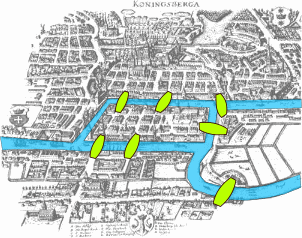
\includegraphics[scale=1]{figs/konigsberg_bridges}
\caption{\label{fig:bridge}%
The city of Königsburg is built on a river and consists of four islands, which can be reached by means of seven bridges.
The question Euler was interested in answering is: Is it possible to go from island to island traversing each bridge only once?
(Picture courtesy of Wikipedia and Wikimedia Commons: \url{http://en.wikipedia.org/wiki/File:Konigsberg_bridges.png}).
}%
\end{figure}
%
\begin{figure}
\centering
\def\grlen{2.7}
\begin{tikzpicture}[%
  nodestyle/.style={
    draw, shape=circle, fill=white,
    blur shadow={shadow blur steps=5}
  }
]
  \node [nodestyle] (A) at (0,0) {A};
  \node [nodestyle] (B) at (0,-\grlen) {B};
  \node [nodestyle] (C) at (0,\grlen) {C};
  \node [nodestyle] (D) at (\grlen,0) {D};

  \graph[
    multi,
    edges={semithick}
  ]{
    {(C),(A),(B)} -- (D);
    (C) --[bend left] (A);
    (C) --[bend right] (A);
    (A) --[bend left] (B) ;
    (A) --[bend right] (B);
  };

  \coordinate (labelpos) at ($(C.north east)+(30:2cm)$);
  \draw[dashed,{Stealth[round,length=3mm]}-] plot [smooth] coordinates{
    (A.north west)
    ($(A.north west)+(140:1cm)$)
    ($(C.north west)+(140:1cm)$)
    (labelpos)
  };
  \node[anchor=west] at (labelpos) {Islands};
  \draw[dashed,{Stealth[round,length=3mm]}-]
    (C.north east) -- ($(labelpos)+(0,-1mm)$);
  \draw[dashed,{Stealth[round,length=3mm]}-]
    (D.north) -- ($(labelpos) + (2mm,-1mm)$);
  \draw[dashed, {Stealth[round,length=3mm]}-] plot [smooth] coordinates{
    (B.east)
    ($(B.east)+(0:15mm)$)
    ($(D.south east)+(-45:8mm)$)
    ($(labelpos)+(7mm,-2mm)$)
  };

  \coordinate (labelpos2) at ($(A.south west) + (-140:2cm)$);
  \draw[dashed,-{Stealth[round, length=3mm]}] (labelpos2) -- ++ (0:1.3cm);
  \node[anchor=east] at (labelpos2) {Bridge};
\end{tikzpicture}
\caption{\label{fig:graphbridges}%
Representing each island as a dot and each bridge as a line or curve connecting the dots simplifies the visual representation of the seven Königsburg Bridges.
}%
\end{figure}
%
\begin{example}
The city of Königsburg exists as a collection of islands connected by bridges as shown in Figure~\ref{fig:bridge}.
The problem Euler wanted to analyze was: Is it possible to go from island to island traversing each bridge only once?
This was assuming that there was no trickery such as using a boat.
Euler analyzed the problem by simplifying the representation to a graph.
Assume that we treat each island as a vertex and each bridge as an line egde.
The resulting graph is illustrated in Figure~\ref{fig:graphbridges}.
\end{example}
%
Note this representation dramatically simplifies the analysis of the problem in so far as we can now focus only on the structural properties of this graph.
It is easy to see (from Figure~\ref{fig:graphbridges}) that each vertex has an odd degree.
More importantly, since we are trying to traverse islands without ever recrossing the same bridge (edge), when we enter an island (say C) we will use one of the three edges.
Unless this is our final destination, we must use another edge to leave C.
Additionally, assuming we have not crossed all the bridges yet, we know we must leave C.
That means that the third edge that touches C must be used to return to C a final time.
Alternatively, we could start at Island C and then return once and never come back.
Put simply, our trip around the bridges of Königsburg had better start or end at Island C.
But Islands (vertices) B and D also have this property.
We cannot start and end our travels over the bridges on Islands C, B and D simultaneously- therefore, no such walk around the islands in which we cross each bridge precisely once is possible.

\begin{definition}{(MultiGraph)}
A graph \(G = (V,E)\) is a multigraph if there are two edges \(e_1\) and \(e_2\) in \(E\) so that \(e_1\) and \(e_2\) are equal as sets.
That is, there are two vertices \(v_1\) and \(v_2\) in \(V\)  so that \(e_1=e_2=\{v_1,v_2\}\).
\end{definition}
\begin{remark}
Note in the definition of graph (Definition~\ref{def:graph}) we were very careful to specify that \(E\) is a collection of one and two element subsets of \(V\) rather than to say that \(E\) was, itself, a set.
This allows us to have duplicate edges in the edge set and thus to define multigraphs.
In Computer Science a set that may have duplicate entries is sometimes called a multiset.
A multigraph is a graph in which \(E\) is a multiset.
\end{remark}

Consider the graph associated with the Bridges of Königsburg Problem.
The vertex set is \(V = \{A, B, C, D\}\).
The edge collection is: \(E = \{\{A,B\},\allowbreak\{A,B\},\allowbreak\{A,C\},\allowbreak\{A,C\},\allowbreak\{A,D\},\allowbreak\{B,D\},\allowbreak\{C,D\}\}\).
This multigraph occurs because there are two bridges connecting island \(A\) with island \(B\) and two bridges connecting island \(A\) with island \(C\).
If two vertices are connected by two (or more) edges, then the edges are simply represented as parallel lines (or arcs) connecting the vertices.

%
%\begin{remark}
%Let \(G = (V,E)\) be a graph.
%There are two degree values that are of interest in graph theory: the largest and smallest vertex degrees usually denoted \(\Delta(G)\) and \(\delta(G)\).
%That is:
%\begin{align}
%  \Delta(G) &= \max\deg(v) v'in V \\
%  \delta(G) &= \min\deg(v) v\in V
%\end{align}
%\end{remark}
%
\begin{remark}\label{rem:simple}
Despite our initial investigation of The Bridges of Königsburg Problem as a mechanism for beginning our investigation of graph theory, most of graph theory is not concerned with graphs containing either self-loops or multigraphs.
\end{remark}
%
\begin{definition}{(Simple Graph)}
A graph \(G = (V,E)\) is a simple graph if \(G\) has no edges that are self-loops and if \(E\) is a subset of two element subsets of \(V\); i.e., G is not a multi-graph.
\end{definition}
%
\begin{remark}
In light of Remark~\ref{rem:simple} and the applications in energy networks which will follow, we will assume that every graph we discuss in these notes is a simple graph and we will use the term graph to mean simple graph.
When a particular result holds in a more general setting, we will state it explicitly.
\end{remark}
%\begin{ex} Consider the new Bridges of Ko ̈nigsburg Problem from Exercise 1.
%Is the graph representation of this problem a simple graph? Could a self-loop exist in a graph derived from a Bridges of Ko ̈nigsburg type problem? If so, what would it mean? If not, why?
%\end{ex}
